\documentclass[UTF8]{ctexart}
\usepackage{../Zhihu}
\usepackage{mhchem}
\title{数字电路学习笔记(十二):时序逻辑设计}
\begin{document}
\maketitle
在了解了这么多时序逻辑的抽象概念之后,我们来研究怎么把它们变成实际可操作的逻辑设计方法论。

一般来说,如果已经给出需求,时序逻辑设计有如下几步:
\begin{enumerate}
\item 把自然语言描述的逻辑抽象化,确定电路状态数,画出状态转换图;
\item 列出三个方程:输出方程、驱动方程、状态方程;
\item 设计具体电路。
\end{enumerate}

直接从具体案例分析。现在的需求是:
\begin{quote}
设计一个自动售饮料机的逻辑电路。它的投币口每次只能投入一枚五角或一元的硬币。累计投入一元五角硬币后机器自动给一杯饮料;投入二元硬币后,在给饮料的同时退回一枚五角的硬币。 \cite{Q1}
\end{quote}

\section*{一、定义变量与状态}
逻辑设计的过程和组合逻辑大致相同,首先要定义各个变量。此处有两个输入:投入五角硬币$A$、投入一元硬币$B$;有两个输出:给饮料$X$、找回五角硬币$Y$。除此之外,时序逻辑除了输入输出,还要定义状态。我们的电路可能有几种状态?在一个完整的服务周期中,它可能处于以下几种状态:
\begin{enumerate}
\item $Q_0$:无投币;
\item $Q_1$:共投入了五角,等待继续投币;
\item $Q_2$:共投入了一元,等待继续投币;
\end{enumerate}

可能在一开始,会觉得投入了一元五角和两元也是状态,但实际上它们并不是可维持的状态。比如当电路处于$Q_2$状态时,一旦再投入一元,就会立刻有输出(给饮料),然后回到“无投币”的基态。因此可以直接把这种情况视作由输入$B=1$导致的输出$X=1,Y=1$,而不是一个瞬时的“投入两元”的状态。

\section*{二、状态转换图与状态编码}
画状态转换图的过程,就是一个“从电路的角度思考”的过程。作为一个电路,我们以极快的频率(比如每秒10次)检测电路的输入,是$AB=00$(无投币),$A=1$(投入五角)还是$B=1$(投入一元),然后根据自身状态决定次态和输出。我们从一个“基态”(比如$Q_0$)出发,每次枚举所有可能的输入,研究它跳转到的状态以及同时给出的输出。画出如下的转换图:
\begin{figure}
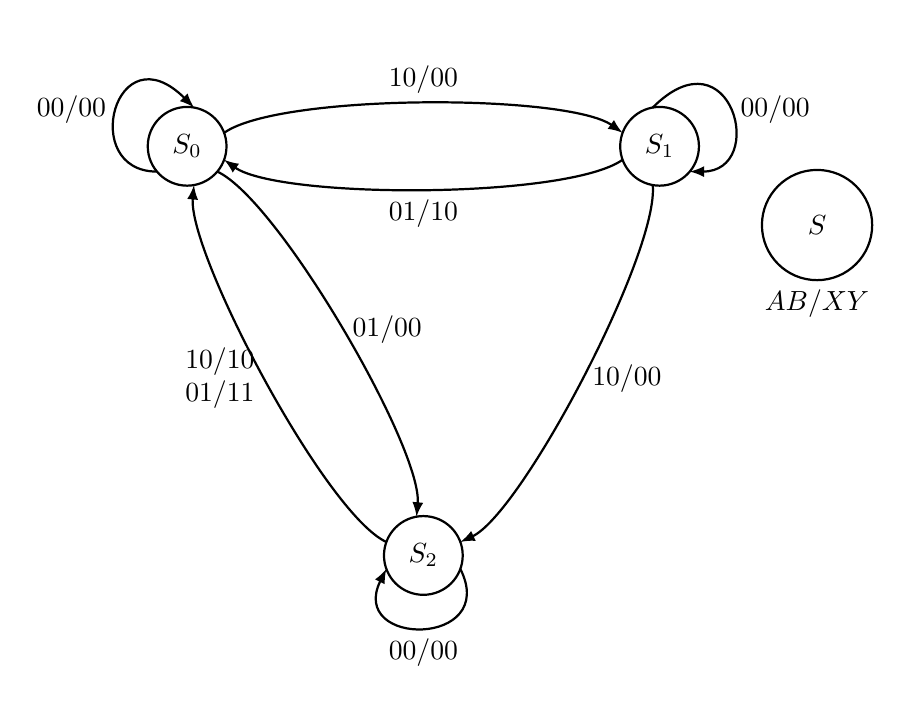
\begin{tikzpicture}[scale=1]
    \tikzset{style={align=center}};
    \draw[thick] (0,0) node {$S_0$} circle[radius=0.5];
    \draw[thick] (6,0) node {$S_1$} circle[radius=0.5];
    \draw[thick] (3,{-sqrt(27)}) node {$S_2$} circle[radius=0.5];
    \draw[-latex,thick] ([shift={(220:0.5)}]0,0) .. controls +(-1,0) and +(-1,1) .. node[left] {$00$/$00$} ([shift={(80:0.5)}]0,0);
    \draw[-latex,thick] ([shift={(20:0.5)}]0,0) .. controls +(0.7,0.5) and +(-0.7,0.5) .. node[above] {$10$/$00$} ([shift={(160:0.5)}]6,0);
    \draw[-latex,thick] ([shift={(-160:0.5)}]6,0) .. controls +(-0.7,-0.5) and +(0.7,-0.5) .. node[below] {$01$/$10$} ([shift={(-20:0.5)}]0,0);
    \draw[-latex,thick] ([shift={(100:0.5)}]6,0) .. controls +(1,1) and +(1,0) .. node[right] {$00$/$00$} ([shift={(-40:0.5)}]6,0);
    \draw[-latex,thick] ([shift={(-100:0.5)}]6,0) .. controls +(0.08,-0.86) and +(0.78,0.36) .. node[right] {$10$/$00$} ([shift={(20:0.5)}]3,{-sqrt(27)});
    \draw[-latex,thick] ([shift={(-20:0.5)}]3,{-sqrt(27)}) .. controls +(0.5,-1) and +(-0.5,-1) .. node[below] {$00$/$00$} ([shift={(-160:0.5)}]3,{-sqrt(27)});
    \draw[-latex,thick] ([shift={(160:0.5)}]3,{-sqrt(27)}) .. controls +(-0.78,0.36) and +(-0.08,-0.86) .. node[left] {$10$/$10$\\$01$/$11$} ([shift={(-80:0.5)}]0,0);
    \draw[-latex,thick] ([shift={(-40:0.5)}]0,0) .. controls +(0.78,-0.36) and +(0.08,0.86) .. node[right] {$01$/$00$} ([shift={(100:0.5)}]3,{-sqrt(27)});
    \draw[thick] (8,-1) node {$S$} circle[radius=0.7];
    \node at (8,-2) {$AB$/$XY$};
\end{tikzpicture}
\end{figure}

这张图一旦自己绘制过一遍,就非常容易理解它的逻辑。每一次投币导致了状态变化,并决定是否产生输出。有一个值得注意的:$S$和$Q$虽然都表示“状态”,但它们不是等价的。$S$表示一个抽象的状态,下标表示状态的编号;$Q$则是具象的,表示状态中的一个比特。比如可能有$S_1=Q_3Q_2Q_1Q_0=0001$。

接下来,把状态编码。由于只有三个状态,并且没有等价状态(也就是相同的输入会导致相同的输出和相同的次态),只要把它们顺序编码即可。我们先用最显然的$S_0=00,S_1=01,S_2=10$,这用2个触发器即可表达。

最后,我们可以把转换图抽象成更适合逻辑分析的卡诺图。

\begin{figure}
\begin{tabular}{rc|c|c|c|}
    \multirow{2}{*}{\backslashbox{$AB$}{$Q_1Q_0$}}&\multicolumn{1}{r}{}&\multicolumn{1}{r}{}&\multicolumn{1}{r}{}&\multicolumn{1}{r}{}\\
    &\multicolumn{1}{c}{\makebox[2em]{00}}&\multicolumn{1}{c}{\makebox[2em]{01}}&\multicolumn{1}{c}{\makebox[2em]{11}}&\multicolumn{1}{c}{\makebox[2em]{10}}\\\cline{2-5}
    \multicolumn{1}{r|}{00}&00/00&01/00&$\times\times$/$\times\times$&10/00\\\cline{2-5}
    \multicolumn{1}{r|}{01}&10/00&00/10&$\times\times$/$\times\times$&00/11\\\cline{2-5}
    \multicolumn{1}{r|}{11}&$\times\times$/$\times\times$&$\times\times$/$\times\times$&$\times\times$/$\times\times$&$\times\times$/$\times\times$\\\cline{2-5}
    \multicolumn{1}{r|}{10}&01/00&10/00&$\times\times$/$\times\times$&00/10\\\cline{2-5}
\end{tabular}
\end{figure}

这样,我们就完成了逻辑抽象的步骤。

\section*{三、列出方程}
再次回忆时序逻辑中的三组方程:
\begin{equation*}
\begin{aligned}
输出方程:Y&=F(X,Q)\\
驱动方程:Z&=G(X,Q)\\
状态方程:Q^*&=H(Z,Q)
\end{aligned}
\end{equation*}
   
我们可以用和组合逻辑几乎一样的思路来得到这些方程,也就是真值表或卡诺图。由于时序逻辑往往有很多无关项(那些不可能出现的状态),卡诺图反倒更加常用。

第二节中给出的卡诺图是一张总图,同时出现了四个因变量(次态$Q_1^*Q_0^*$和输出$XY$),但如果要用卡诺图合并同类项,我们就只能一次处理一个变量。因此把总图拆成四张子图:

\begin{figure}
\begin{tabular}{rc|c|c|c|}
    \multirow{2}{*}{\backslashbox{$AB$}{$Q_1Q_0$}}&\multicolumn{1}{r}{}&\multicolumn{1}{r}{}&\multicolumn{1}{r}{}&\multicolumn{1}{r}{}\\
    &\multicolumn{1}{c}{\makebox[2em]{00}}&\multicolumn{1}{c}{\makebox[2em]{01}}&\multicolumn{1}{c}{\makebox[2em]{11}}&\multicolumn{1}{c}{\makebox[2em]{10}}\\\cline{2-5}
    \multicolumn{1}{r|}{00}&0&0&$\times$\tikzmark{circ2start}&1\tikzmark{circ2end}\\\cline{2-5}
    \multicolumn{1}{r|}{01}&1\tikzmark{circ3start}&0&$\times$&0\\\cline{2-5}
    \multicolumn{1}{r|}{11}&$\times$\tikzmark{circ3end}&$\times$\tikzmark{circ1start}&$\times$&$\times$\\\cline{2-5}
    \multicolumn{1}{r|}{10}&0&1&$\times$\tikzmark{circ1end}&0\\\cline{2-5}
\end{tabular}
\begin{tikzpicture}[remember picture,overlay]
    \draw[rounded corners=10pt,thick,dashed]
    ([shift={(-\tabcolsep-1em+0.5ex,2ex)}]pic cs:circ1start) rectangle
    ([shift={(1em-0.7ex,-0.8ex)}]pic cs:circ1end);
    \draw[rounded corners=5pt,thick,dashed]
    ([shift={(-\tabcolsep-1em+0.5ex,2ex)}]pic cs:circ2start) rectangle
    ([shift={(1em-0.7ex,-0.8ex)}]pic cs:circ2end);
    \draw[rounded corners=5pt,thick,dashed]
    ([shift={(-1em+0.5ex,2ex)}]pic cs:circ3start) rectangle
    ([shift={(1em-2ex,-0.8ex)}]pic cs:circ3end);
\end{tikzpicture}
\caption*{$Q_1^*$}
\end{figure}
\begin{figure}
\begin{tabular}{rc|c|c|c|}
    \multirow{2}{*}{\backslashbox{$AB$}{$Q_1Q_0$}}&\multicolumn{1}{r}{}&\multicolumn{1}{r}{}&\multicolumn{1}{r}{}&\multicolumn{1}{r}{}\\
    &\multicolumn{1}{c}{\makebox[2em]{00}}&\multicolumn{1}{c}{\makebox[2em]{01}}&\multicolumn{1}{c}{\makebox[2em]{11}}&\multicolumn{1}{c}{\makebox[2em]{10}}\\\cline{2-5}
    \multicolumn{1}{r|}{00}&0&1\tikzmark{circ4start}&$\times$\tikzmark{circ4end}&0\\\cline{2-5}
    \multicolumn{1}{r|}{01}&0&0&$\times$&0\\\cline{2-5}
    \multicolumn{1}{r|}{11}&$\times$\tikzmark{circ5start}&$\times$&$\times$&$\times$\\\cline{2-5}
    \multicolumn{1}{r|}{10}&1\tikzmark{circ5end}&0&$\times$&0\\\cline{2-5}
\end{tabular}
\begin{tikzpicture}[remember picture,overlay]
    \draw[rounded corners=5pt,thick,dashed]
    ([shift={(-\tabcolsep-1em+0.5ex,2ex)}]pic cs:circ4start) rectangle
    ([shift={(1em-0.7ex,-0.8ex)}]pic cs:circ4end);
    \draw[rounded corners=5pt,thick,dashed]
    ([shift={(-1em+0.2ex,2ex)}]pic cs:circ5start) rectangle
    ([shift={(1em-1.7ex,-0.8ex)}]pic cs:circ5end);
\end{tikzpicture}
\caption*{$Q_0^*$}
\end{figure}
\begin{figure}
\begin{tabular}{rc|c|c|c|}
    \multirow{2}{*}{\backslashbox{$AB$}{$Q_1Q_0$}}&\multicolumn{1}{r}{}&\multicolumn{1}{r}{}&\multicolumn{1}{r}{}&\multicolumn{1}{r}{}\\
    &\multicolumn{1}{c}{\makebox[2em]{00}}&\multicolumn{1}{c}{\makebox[2em]{01}}&\multicolumn{1}{c}{\makebox[2em]{11}}&\multicolumn{1}{c}{\makebox[2em]{10}}\\\cline{2-5}
    \multicolumn{1}{r|}{00}&0&0&$\times$&0\\\cline{2-5}
    \multicolumn{1}{r|}{01}&0&1\tikzmark{circ6start}&$\times$\tikzmark{circ7start}&1\\\cline{2-5}
    \multicolumn{1}{r|}{11}&$\times$&$\times$&$\times$\tikzmark{circ8start}\tikzmark{circ6end}&$\times$\tikzmark{circ7end}\\\cline{2-5}
    \multicolumn{1}{r|}{10}&0&0&$\times$&1\tikzmark{circ8end}\\\cline{2-5}
\end{tabular}
\begin{tikzpicture}[remember picture,overlay]
    \draw[rounded corners=10pt,thick,dashed]
    ([shift={(-\tabcolsep-1em+0.5ex,2ex)}]pic cs:circ6start) rectangle
    ([shift={(1em-0.7ex,-0.8ex)}]pic cs:circ6end);
    \draw[rounded corners=10pt,thick,dashed]
    ([shift={(-\tabcolsep-1em+0.5ex,2ex)}]pic cs:circ7start) rectangle
    ([shift={(1em-0.7ex,-0.8ex)}]pic cs:circ7end);
    \draw[rounded corners=10pt,thick,dashed]
    ([shift={(-\tabcolsep-1em+0.6ex,2ex)}]pic cs:circ8start) rectangle
    ([shift={(1em-0.5ex,-0.8ex)}]pic cs:circ8end);
\end{tikzpicture}
\caption*{$X$}
\end{figure}
\begin{figure}
\begin{tabular}{rc|c|c|c|}
    \multirow{2}{*}{\backslashbox{$AB$}{$Q_1Q_0$}}&\multicolumn{1}{r}{}&\multicolumn{1}{r}{}&\multicolumn{1}{r}{}&\multicolumn{1}{r}{}\\
    &\multicolumn{1}{c}{\makebox[2em]{00}}&\multicolumn{1}{c}{\makebox[2em]{01}}&\multicolumn{1}{c}{\makebox[2em]{11}}&\multicolumn{1}{c}{\makebox[2em]{10}}\\\cline{2-5}
    \multicolumn{1}{r|}{00}&0&0&$\times$&0\\\cline{2-5}
    \multicolumn{1}{r|}{01}&0&0&$\times$\tikzmark{circ9start}&1\\\cline{2-5}
    \multicolumn{1}{r|}{11}&$\times$&$\times$&$\times$&$\times$\tikzmark{circ9end}\\\cline{2-5}
    \multicolumn{1}{r|}{10}&0&0&$\times$&0\\\cline{2-5}
\end{tabular}
\begin{tikzpicture}[remember picture,overlay]
    \draw[rounded corners=10pt,thick,dashed]
    ([shift={(-\tabcolsep-1em+0.5ex,2ex)}]pic cs:circ9start) rectangle
    ([shift={(1em-0.7ex,-0.8ex)}]pic cs:circ9end);
\end{tikzpicture}
\caption*{$Y$}
\end{figure}

这样就不难得到输出方程和状态方程。
\begin{equation*}
\begin{aligned}
&\begin{cases}
X=Q_0B+Q_1B+Q_1A\\
Y=Q_1B
\end{cases}\\
&\begin{cases}
Q_1^*=Q_1'Q_0'B+Q_1A'B'+Q_0A\\
Q_0^*=Q_0A'B'+Q_1'Q_0'A
\end{cases}
\end{aligned}
\end{equation*}

但为了确定驱动方程,表示出内部输入$Z$,我们要先决定用什么触发器。最常用的是JK触发器和D触发器。前者功能更加强大,后者则在设计时更简单,但很可能最终逻辑更复杂。回忆它们的特性方程分别是:
\begin{equation*}
\begin{aligned}
Q^*&=J\cdot Q'+K'\cdot Q\\
Q^*&=D
\end{aligned}
\end{equation*}

其中$J,K,D$等便是内部输入。比如,如果我们选用JK触发器设计电路,就可以将特性方程和状态方程作比较:
\begin{equation*}
\begin{cases}
Q_1^*=Q_1'Q_0'B+Q_1A'B'+Q_0A\\
Q_0^*=Q_0A'B'+Q_1'Q_0'A
\end{cases}\Longleftrightarrow\begin{cases}
Q_1^*=J_1\cdot Q_1'+K_1'\cdot Q_1\\
Q_0^*=J_0\cdot Q_0'+K_0'\cdot Q_0
\end{cases}
\end{equation*}

我们要把$Q'_i$和$Q_i$对应的系数作为$J_i$和$K'_i$。可以略微改写一下:
\begin{equation*}
\begin{cases}
Q_1^*=(Q_0'B+Q_0A)Q_1'+(A'B'+Q_0A)Q_1\\
Q_0^*=(A'B')Q_0+(Q_1'A)Q_0'
\end{cases}\Longleftrightarrow\begin{cases}
Q_1^*=J_1\cdot Q_1'+K_1'\cdot Q_1\\
Q_0^*=J_0\cdot Q_0'+K_0'\cdot Q_0
\end{cases}
\end{equation*}

从而得到驱动方程:
\begin{equation*}
\begin{cases}
J_1=Q_0'B+Q_0A\\
K_1=(A'B'+Q_0A)'=Q_0A+B\\
J_0=Q_1'A\\
K_0=(A'B')'=A+B
\end{cases}
\end{equation*}

而如果选用了D触发器,那么由于$Q^*=D$,只要把对应的$Q^*_i$改写成$D^*$即可:
\[\begin{cases}
D_1=Q_1'Q_0'B+Q_1A'B'+Q_0A\\
D_0=Q_0A'B'+Q_1'Q_0'A
\end{cases}\]

可以看到,JK触发器得到的最终方程更简单。

\section*{四、画电路图}
这是我们的电路图的抽象。

\begin{figure}
\begin{circuitikz}[scale=1, transform shape]
    \ctikzset{multipoles/dipchip/width=1.7}
    \node[flipflop JK] (j1) at (0,0) {};
    \node[flipflop JK] (j2) at (0,-4) {};
    \node[dipchip,hide numbers,no topmark] (x) at (-4,-2) {$Z=G(X,Q)$};
    \node[dipchip,hide numbers,no topmark,external pins width=0] (y) at (-4,2) {$Y=F(X,Q)$};
    \draw (x.pin 8) node[above] {$J_1$} -| ([xshift=-1cm]j1.pin 1) -- (j1.pin 1);
    \draw (x.pin 7) node[above] {$K_1$} -| ([xshift=-0.5cm]j1.pin 3) -- (j1.pin 3);
    \draw (x.pin 6) node[above] {$J_0$} -| ([xshift=-0.5cm]j2.pin 1) -- (j2.pin 1);
    \draw (x.pin 5) node[above] {$K_0$} -| ([xshift=-1cm]j2.pin 3) -- (j2.pin 3);
    \draw (j1.pin 6) -| ++(0.5,3) -- ++(-7.5,0) |- (x.pin 3);
    \draw (j2.pin 6) -| ++(1,7.5) -- ++(-8.5,0) |- (x.pin 4);
    \draw (x.pin 1) -- ++(-1.5,0) |- (y.pin 1);
    \draw (x.pin 2) -- ++(-2,0) |- (y.pin 2);
    \draw (y.pin 3) to[short,-*] ++(-0.7,0);
    \draw (y.pin 4) to[short,-*] ++(-1.2,0);
    \draw (y.pin 7) -- ++(6,0) node[above] {$X$};
    \draw (y.pin 6) -- ++(6,0) node[above] {$Y$};
    \draw ([xshift=-1.5cm]x.pin 1) node[circ] {} -- ++(-1.5,0) node[above] {$A$};
    \draw ([xshift=-2cm]x.pin 2) node[circ] {} -- ++(-1,0) node[above] {$B$};
\end{circuitikz}
\end{figure}

由于已经有了输出方程$Y=F(X,Q)$和驱动方程$Z=G(X,Q)$,分别是
\[\begin{cases} X=Q_0B+Q_1B+Q_1A\\ Y=Q_1B \end{cases}和\begin{cases} J_1=Q_0'B+Q_0A\\ K_1=(A'B'+Q_0A)'=Q_0A+B\\ J_0=Q_1'A\\ K_0=(A'B')'=A+B \end{cases},\]
可以直接把它们的方程代入,画出电路。

\begin{thebibliography}{5}
    \bibitem{Q1} 数字电路与逻辑设计,张俊涛著,清华大学出版社2017版
\end{thebibliography}
\end{document}
